\documentclass[11pt,a4paper]{article}
\usepackage[T1]{fontenc}
\usepackage[utf8]{inputenc}
\usepackage[margin=25mm]{geometry}
\usepackage{lmodern,microtype,amsmath,amssymb,booktabs,tikz,hyperref}
\usetikzlibrary{arrows.meta}
\hypersetup{colorlinks=true,urlcolor=teal!60!black}
\setlength{\parindent}{0pt}
\setlength{\parskip}{4pt}
\newcommand{\ord}{\operatorname{ord}}
\newcommand{\Disc}{\operatorname{Disc}}
\begin{document}
\begin{center}
{\Large\bfseries Multiplicity in a phase average of the Hurwitz shift\\and in two prime periods}\\[4pt]
{\small Research note, 23 November 2026. OpenAI Codex.}
\end{center}

The September split-zero construction recovers an entire compact measure from the local polynomial of a
Hurwitz zero cluster (historical Hurwitz jets, H10--H13). The November signed-motion calculation gives
fractional-power branches and a residue formula for the ordinary shift (NEG\_NIGHT NN-A005).
The prime-period construction retains each finite spectral jet under $s\mapsto p^{s-1/2}$ (J1--J4).
Combining these constructions gives a multiplicity test in the phase variable itself.

\textbf{Phase average.} For any integer $d\ge1$, set $\xi=\exp(2\pi i/d)$ and, for $|t|<1$, define
\[
 H_d(s,t)=\frac1d\sum_{j=0}^{d-1}\zeta(s,1+\xi^jt).
\]
Use the branch continued from the positive base at $t=0$. The power series is holomorphic jointly near any
nontrivial zero $\rho$ of $\zeta$. Only powers $t^{dh}$ survive the finite Fourier average, so
\[
 H_d(s,t)=\zeta(s)+b_d(s)t^d+O(t^{2d}),\qquad
 b_d(s)=(-1)^d\frac{(s)_d}{d!}\zeta(s+d),
\]
where $(s)_d=s(s+1)\cdots(s+d-1)$. This follows by expanding each $(n+\xi^jt)^{-s}$ first for
$\Re s>1$ and then continuing the Taylor coefficients in $s$. Equivalently one can differentiate
the Hurwitz shift in its second argument. At every nontrivial zero $b_d(\rho)\ne0$, since
$\Re(\rho+d)>1$ and the other factors are nonzero.

\textbf{Proposition.} If $\rho$ has multiplicity $m$, the monic equation for the $m$ nearby zeros has
discriminant of order exactly $d(m-1)$ in $t$. On taking one small positive circuit in $t$, the branch
permutation has $\gcd(m,d)$ cycles, each of length $m/\gcd(m,d)$.

\textit{Proof.} Write $a=\zeta^{(m)}(\rho)/m!$. Regard $H_d$ as a function of $s$ and $u=t^d$, and write
$u=w^m$, $s=\rho+wz$. Division by $w^m$ gives $az^m+b_d(\rho)+O(w)$ near each root of the leading polynomial.
Its roots are distinct, since $a b_d(\rho)\ne0$. The implicit function theorem continues them analytically
in $w$, and a small fixed circle about $\rho$ retains exactly $m$ zeros by the argument principle. Thus on
a chosen branch
\[
 s_j(t)=\rho+c\,e^{2\pi ij/m}t^{d/m}+O(t^{2d/m}),\qquad c^m=-b_d(\rho)/a .
\]
Every pair difference has a nonzero leading coefficient. Squaring and multiplying the $\binom m2$ differences
gives order $d(m-1)$; the product is single-valued by symmetry. A circuit of $t$ advances the index by $d$
modulo $m$. The assertion includes $m=1$, with discriminant one and a stationary branch label. \hfill$\square$

\begin{center}
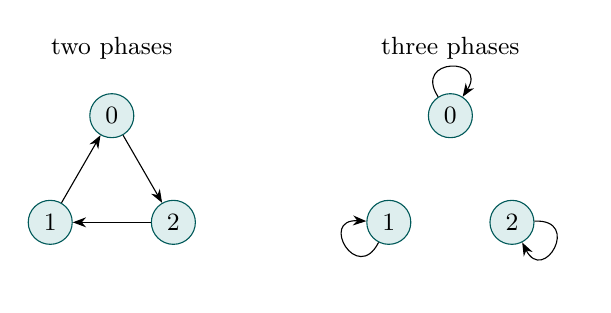
\begin{tikzpicture}[>=Stealth,scale=.86,font=\small]
\foreach \x/\n/\l in {0/2/{two phases},5/3/{three phases}}{
  \begin{scope}[shift={(\x,0)}]
  \node at (0,2.05) {\l};
  \foreach \a/\j in {90/0,210/1,330/2}{
    \node[circle,fill=teal!13,draw=teal!70!black,inner sep=3pt] (P\j) at (\a:1.05) {\j};}
  \ifnum\n=2
    \draw[->] (P0) -- (P2);
    \draw[->] (P2) -- (P1);
    \draw[->] (P1) -- (P0);
  \else
    \foreach \a/\j in {90/0,210/1,330/2}{
      \path[->] (P\j) edge[out=\a+33,in=\a-33,loop,looseness=4,min distance=7mm] (P\j);}
  \fi
  \end{scope}}
\end{tikzpicture}\\
{\small A triple zero. The dots label analytic branches. One circuit of $t$ acts by $j\mapsto j+d$
modulo three. Arrows indicate continuation, not distances in the $s$-plane.}
\end{center}

\newpage
\textbf{A fixed contour.} Take disjoint small disks around the $r$ distinct enclosed zeros of $\zeta$ with
multiplicities $m_1,\ldots,m_r$. Let $M=\sum m_i$, and choose the contour free of zeros and poles. For small
$t$ the cluster polynomials can be obtained without choosing branches, by contour power sums and Newton's
identities. Differences between roots coming from distinct disks have nonzero limits. Therefore the discriminant
of the full monic polynomial satisfies
\[
 \ord_{t=0}\Disc_s=d\sum_{i=1}^r(m_i-1)=d(M-r).
\]
For a single disk this gives the individual multiplicity. For a union it gives the excess of multiplicity over the
number of distinct zeros. Two double zeros and a triple plus a simple zero both have excess two. The subdiscriminants
of the backward heat flow in the companion paper read the complete partition on such a union. The two degrees
$d=2,3$ additionally distinguish the monodromies of an individual double or triple zero.

\textbf{Reading the same excess after taking a prime period.} For a rational prime $p$ use the unmarked map
$z_p(s)=p^{s-1/2}$. A single common nonzero phase multiplying $z_p$ is harmless.
Write $\Delta_p(t)$ for the discriminant of the monic polynomial of all $M$ images, counted with multiplicity.
Then
\[
 d(M-r)=\min_{p\in\mathcal P}\ord_{t=0}\Delta_p(t)
 \quad\text{for any set of }\binom M2+1\text{ distinct rational primes}.
\]
The empty and one-root cases use the usual discriminant convention. An identically vanishing discriminant has
order $+\infty$.

\textit{Proof.} The derivative of $z_p$ is $(\log p)z_p$, everywhere nonzero. Consequently the image differences
within a disk have exactly the orders computed on the first page. Cross-disk pairs add a nonnegative order.
Equality holds for a prime separating the $r$ centres. Two distinct centres $\rho_i,\rho_j$ can collide for
at most one rational prime. Indeed a collision at $p$ gives $(\rho_i-\rho_j)\log p=2\pi i k$ with $k$ a
nonzero integer. Collision at another prime $p'$ would give $\log p/\log p'\in\mathbb Q$, contrary to unique
factorization. At most $\binom r2$ primes are bad, and $\binom r2\le\binom M2$. All the image coefficients are
holomorphic in $t$ by symmetry, or directly by contour integration against powers of $z_p$. \hfill$\square$

Under Alpöge's RH the undeformed centres of these prime periods all have modulus one. The local multiplicity
and monodromy calculations themselves use only $0<\Re\rho<1$. They provide a finite-contour consequence of the
older split-zero construction under its actual hypotheses. To turn the test into a finite-precision certificate
one needs a lower bound on nonzero discriminants or separation with a controlled remainder. To deduce global
simplicity one would additionally need a theorem excluding collisions at every height.

\medskip
\textit{Sources.} \emph{Historical Hurwitz reconstruction and the complete Laurent jet bridge}, H1--H2, H10--H13
and J1--J4. \emph{All shifted-series jets and factorization obstruction}, NN-A004--005 in
\texttt{shift\_jets.tex}. For the Hurwitz derivative see
\href{https://dlmf.nist.gov/25.11.E17}{NIST DLMF 25.11.17}. For the RH input see
\href{https://alpo.ge/remark.pdf}{Alpöge's announcement} and
\href{https://math.mit.edu/~drew/grh/}{Sutherland's verification records}. The root-of-unity average and
the separating-prime discriminant formula above are the deductions on pp.~1--2.

\newpage
\section*{An integer multiplicity from two prime periods}
In the original two-prime theorem (P1--P4), the paired period coordinates separate all complex
centres and preserve the full local algebra. Under RH each ordinate $\gamma_j$ on a fixed contour
now gives a point $(p^{i\gamma_j},q^{i\gamma_j})$ on two unit circles, carrying a positive integer
mass $m_j$. The same finite table can measure the mass in several prescribed height intervals.

Fix distinct rational primes $p,q$ and write $a=\log p,\ b=\log q$. A positively oriented contour
$\Gamma$ in the open critical strip encloses $M=\sum_j m_j$ zeros and meets none. Its mixed moments are
\[
 S_{kl}=\sum_j m_j e^{i(ka+lb)\gamma_j}
 =\frac1{2\pi i}\int_\Gamma e^{(s-1/2)(ka+lb)}
                 \frac{\zeta'(s)}{\zeta(s)}\,ds .
\]
The identity follows from the residue theorem. The first equality uses the critical line. Let the
target ordinates lie within $h$ of a supplied $\gamma_0$. All other enclosed ordinates have distance
in $[\Delta,H]$ from $\gamma_0$, where $0\le h<\Delta\le H<\infty$. Write $m$ for the total target mass.
For $K\ge2$ use $w_k=(K-|k|)/K^2$ for $|k|<K$. Given moment errors
$|\widetilde S_{kl}-S_{kl}|\le\epsilon$, set
\[
 A=\Re\sum_{|k|,|l|<K} w_k w_l e^{-i(ka+lb)\gamma_0}\widetilde S_{kl},\qquad
 \sigma=\min_{\Delta\le x\le H}\max\{|e^{iax}-1|,|e^{ibx}-1|\}.
\]
\textbf{Rounding theorem.} The separation $\sigma$ is positive and one has
\[
 |A-m|\ \le\ \epsilon+
 \frac{M(K^2-1)(a^2+b^2)h^2}{12}+
 \frac{4M}{K^2\sigma^2}.
\]
Whenever the right side is less than $1/2$, the nearest integer to $A$ gives the exact mass. In an
interval enclosing one distinct ordinate this is its order as a zero. The formula also applies
to an empty interval and to intervals enclosing several distinct ordinates.

\textit{Proof.} The normalized Fejér kernel is
\[
 F_K(x)=K^{-2}\Big|\sum_{n=0}^{K-1}e^{inx}\Big|^2
       =\sum_{|k|<K}w_ke^{ikx}.
\]
It lies in $[0,1]$, is one at zero and is at most $4/(K^2|1-e^{ix}|^2)$ away from it by the
geometric-series formula. Moreover
$1-F_K(x)\le(K^2-1)x^2/12$, by averaging
$1-\cos((u-v)x)\le (u-v)^2x^2/2$ over $0\le u,v<K$.
The exact data give the sum of $m_j F_K(a(\gamma_j-\gamma_0))F_K(b(\gamma_j-\gamma_0))$.
The quadratic estimate bounds the deficit on the target, and the geometric estimate bounds the
leakage from the other ordinates. The weights are nonnegative and sum to one, so the errors on the
moments contribute at most $\epsilon$. A common zero of $e^{iax}-1$ and $e^{ibx}-1$ with
$x>0$ would make $\log p/\log q$ rational. Compactness now gives $\sigma>0$. \hfill$\square$

\newpage
\section*{What separation buys}
The constants in the rounding theorem can be certified from supplied bounds on the target
interval and on its distance from the other enclosed ordinates. On $[\Delta,H]$ the function
defining $\sigma$ is Lipschitz with constant $\max(a,b)$. Subdivide the interval, take certified
lower bounds for its values at the midpoints, and subtract $\max(a,b)$ times the largest half-width.
Refining the grid and the evaluation precision eventually gives a positive lower bound.
This supplies the separation of the two phase coordinates even if one prime identifies two ordinates.

\begin{center}
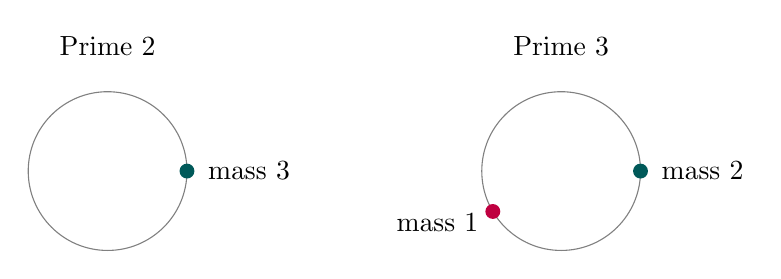
\begin{tikzpicture}[scale=.96]
  \foreach \x/\pr in {0/2,6/3}{
    \begin{scope}[shift={(\x,0)}]
    \node at (0,1.65) {Prime \(\pr\)};
    \draw[gray] (0,0) circle (1.05);
    \fill[teal!70!black] (0:1.05) circle (2.8pt);
    \ifnum\pr=2
      \node[anchor=west] at (1.2,0) {mass 3};
    \else
      \node[anchor=west] at (1.2,0) {mass 2};
      \fill[purple] (210.5865:1.05) circle (2.8pt);
      \node[anchor=east] at (215:1.18) {mass 1};
    \fi
    \end{scope}}
\end{tikzpicture}
\end{center}
In this finite model the ordinates are $0$ (mass two) and $2\pi/\log2$ (mass one). The first prime
puts both at $1$. The second puts the latter at $\exp(2\pi i\log3/\log2)$. Its chordal distance
from $1$ exceeds $1.9$ since $3/2<\log3/\log2<8/5$ and
$2\sin(3\pi/5)=\sqrt{(5+\sqrt5)/2}>1.9$. At either exact target the
leakage is at most $4M/(16^2\cdot1.9^2)<0.014$ for $K=16$. The same joint table therefore reads
both integer masses even with an absolute error $0.1$ in every entry. Here the separation
uses the known other ordinate directly, equivalently $\Delta=H=2\pi/\log2$.

\textbf{The information needed to distinguish two close ordinates.}
For a double atom at $\gamma$ and two unit atoms at $\gamma\pm t$, the difference of the $(k,l)$
moments has magnitude
\[
 2|1-\cos((ka+lb)t)|\le (K-1)^2(a+b)^2t^2,\qquad |k|,|l|<K.
\]
Thus a fixed finite table at positive absolute noise tolerance admits arbitrarily close model
packets with different multiplicity partitions. This gives an obstruction in the class of
positive critical-line measures. Ruling out either packet for actual zeta zeros requires
information about $\zeta$ beyond that tolerance. The rounding theorem gives the total multiplicity
in each prescribed interval satisfying its error bound. A certificate that a narrow interval
contains a single distinct ordinate is an additional input when reading an individual order.

\textit{Sources.} The joint algebra and its proof of separation are P1--P4 in
\emph{Historical Hurwitz reconstruction and the complete Laurent jet bridge}.
The Fejér kernel and its finite Fourier expansion are classical. For recovery of separated point
sources by convex methods see \href{https://arxiv.org/abs/1203.5871}{E.~Candès and C.~Fernandez-Granda,
\emph{Towards a Mathematical Theory of Super-Resolution}}. The calculation here estimates an
integer mass at a supplied interval from the two arithmetic periods and the indicated contour.
\end{document}
